\documentclass[a4paper,12pt]{article}
\usepackage[T1]{fontenc}
\usepackage{imakeidx}
\usepackage{graphicx}
%\makeindex[columns=3, title=Alphabetical Index, intoc]

\begin{document}

\textbf{ISO}


\tableofcontents
\clearpage

 
\section{Introduction}
The International Organization for Standardization is an international standard-setting body composed of representatives from various national standards organizations.

The organization develops and publishes worldwide technical, industrial and commercial standards

\section{TCP-IP vs ISO}

ISO holds lots of standards and when it comes to network it classifies 7 layers whereas TCP/IP (for practical reasons) has only 4 because 3 layers of the standard ISO are actually representing the same physical reality

Here goes a quick example.

It's called ISO/OSI and stands for Open Systems Interconnection Protocolo and it's regulated by the International Organization of Standardization 
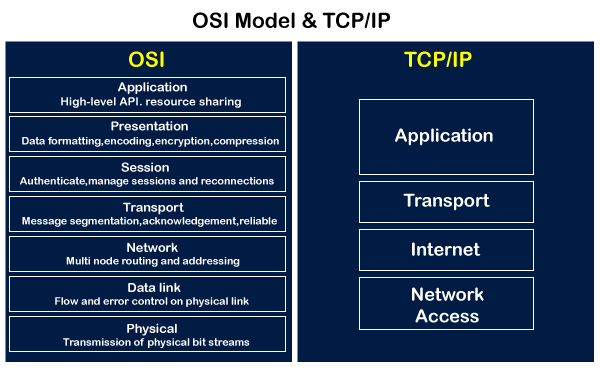
\includegraphics[width=15cm]{./osi-vs-tcp-ip2.png}

\section{ISMS 27001 }

ISO/IEC 27001 is widely known, providing requirements for an information security management system (ISMS).
It enables organizations manage the security of  \emph{assets} such as financial information, intellectual property, employee details or information entrusted by third parties

\subsection{ISO 22301 and differences}

ISO 22301 is an internationally recognised standard that is designed to allow businesses to implement, maintain and improve a business continuity management system (BCMS). The ISO 22301 standard helps you understand and prioritise threats to your organisation. Its BCMS specifies the steps you need to take to reduce the threat of disruption, protect your assets if something does go wrong, and recover quickly from any incidents.

ISO 27001 is much more prescriptive, with organisations required to choose which of the
information security control objectives and controls should apply to their organisation and to justify
any exclusions that they chose to adopt, and then deciding how they would implement any controls,
with detailed guidance given in ISO 27002.


\section{Environmental 14001}
ISO 14001 sets the standard for Environmental Management Systems.

If you want to reduce waste management costs and demonstrate your commitment to protecting the environment, you need ISO 14001 certification. Implementing this global standard will also help you building trust with customers.

\section{Quality 9001}
ISO 9001 is used by businesses to continually monitor, manage and improve the quality of their products and services.

It is a powerful business improvement tool, providing the framework and guidance you need to help you consistently meet your customer’s expectations and regulatory requirements.

\clearpage

\printindex

\section{BCM}
Business continuity management (BCM) is defined in ISO 22301:2012 as “an holistic management process that identifies potential threats to an organization and the impacts to business operations those threats, if realized, might cause, and which provides a framework for building organizational resilience with the capability of an effective response that safeguards the interests of its key stakeholders, reputation, brand and value-creating activities”.

\subsection{ Impact analysis }
The impact analysis phase consists of:

\begin{itemize}
\item \textbf{Business impact analysis (BIA)}: differentiating between critical (urgent) and non-critical (non-urgent) organisational functions, and determining the recovery requirements for each critical function.
\item \textbf{Threat and risk analysis (TRA)}: determining any unique recovery steps that may be required to respond to each potential threat.
In addition, impact scenarios should be considered and documented for each identified threat.
\end{itemize}

\subsection{Solution design}
The solution design phase identifies the most cost-effective disaster recovery solution that meets the main requirements from the impact analysis stage, and determines:

\begin{itemize}
\item Crisis management command structure
\item Secondary work sites
\item Data replication methodology between primary and secondary work sites
\item Applications and data required at the secondary work site
\end{itemize}

\subsection{Implementation}
This stage of the lifecycle concentrates on executing the agreed strategies and tactics through the process of developing a business continuity plan (BCP).

\subsection{Testing and organisational acceptance}
The purpose of testing is to make sure it meets the organisation’s requirements.

The 2008 book Exercising for Excellence, published by the British Standards Institution, identified three types of exercises for testing BCPs:

\begin{itemize}
\item \textbf{Tabletop exercises}: Typically involving a small number of people, tabletop exercises tend to concentrate on a specific aspect of a BCP.
\item \textbf{Medium exercises}: A medium exercise is conducted within a \emph{virtual world} and typically concentrates on multiple BCP aspects, prompting interaction between teams. Realism may extend to simulated news broadcasts and websites.
\item \textbf{Complex exercises}: A complex exercise incorporates all the aspects of a medium exercise and aims to have as few boundaries as possible. Exercises might include no-notice activation, actual evacuation and actual invocation of a disaster recovery site.
\end{itemize}

\subsection{Maintenance}
Maintenance of a BCP ensures that plans remain aligned with current business practices, and can be broken down into three periodic activities:

\begin{itemize}
\item Confirmation of information, roll out to staff for awareness and specific training for critical individuals.
\item Testing and verification of technical solutions established for recovery operations.
\item Testing and verification of organisational recovery procedures.
\end{itemize}
Issues identified in the testing phase often need to be reconsidered as part of the impact analysis phase.

Following the BCM lifecycle guarantees your organisation can continue to deliver its key products and services during a disaster, and ensures that it survives thereafter.


\end{document}
